\mainmatter
% Partie 1: présentation du personnage
\chapter{La Vie, le Jazz, le Verbe}\footnote{L'emploi de majuscules, ici,
n'est ni fortuit, ni une basse erreur typographique (Faustroll m'en préserve !). Ces trois mots ont été nomproprifiés (en utilisant un détergent du
meilleur tonneau, préservant les couleurs) à dessein et sans scrupule,
étant donné l'importance de ce qu'ils représentent avaient pour le sujet du
présent document.}
\epigraph{%
Je n'ai pas besoin de gagner ma vie, puisque je l'ai déjà.}{Boris Vian}
\vfill
\pagebreak
%\section{\BV, Bison \bsc{Ravi}, et tous leurs amis}
%\section{{\sout{Une}} Des vie{\uline{s}} bien remplie{\uline{s}}}
\section{Des vies bien remplies}
\epigraph{Romancier, poète, dramaturge, ingénieur, trompettiste, auteur
de chansons et de film, directeur artistique de maisons de disques, pataphysicien, roi
de Saint-Germain-des-Prés\ldots Ce sont bien mille et une vies que Boris Vian sera parvenu
à vivre en trente-neuf ans d'existence.}
{\emph{Les Vies parallèles de Boris Vian}, Noël \bsc{Arnaud}, quatrième de couverture}

% Intro

\lettrine{I}l est difficile de parler de \BV. Peut-être parce qu'il
est difficile de lui coller une seule étiquette. Un seul nom,
même. « \BV\ » pour l'état civil, « Bison \bsc{Ravi} » --- anagramme
de « \BV\ » pour les proches, « Vernon \bsc{Sullivan} » pour certains
livres, et des dizaines d'autres pseudonymes en tant que chroniqueur.
% TODO: lien liste des pseudonymes (annexes ?)
Mais pour évoquer le personnage, on peut déjà s'intéresser à l'Histoire,
et à son histoire.

% TODO: Annexe frise chrono ?

\subsection{Contexte historique}
Il est nécessaire de décrire le contexte historique de la vie
de \BV\ pour comprendre certaines forces externes qui
ont pu avoir une influence significative sur sa vie, ainsi que
sur son oeuvre.

\BV\ est né peu après la seconde guère mondiale. En \nb{1929}, c'est
la crise avec le crash de Wall Street. En \nb{1940}, l'Allemagne envahit la
partie nord de la France. Toute une partie de la culture est alors
interdite et censurée, notament le jazz, d'origine noire-américaine.

\subsection{Famille et éducation}

\BV \ est issu d'une famille riche. Son père, Paul \bsc{Vian}, est rentier
depuis ses \nb{20} ans. Sa mère est l'héritière d'une riche famille de l'industrie
du papier.

Les Vian habitent une grande maison, «Les Fauvettes», à Ville d'Avray, dans la
banlieue de Paris, près du parc de Saint-Cloud. Le plus important est le loisir,
le divertissement, tout ce qui est agréable. Les enfants Vian vivent ainsi coupés
du monde extérieur: la politique, la religion, ou tout autre sujet sérieux n'entre
pas dans ce petit monde clos. On profite de la vie.

Cette maison n'est pas le seul paradis des Vian. Tous les étés, ils se rendent
à Landemer, dans le Cotentin, où les enfants peuvent jouer tout l'été sur la
plage privée de la propriété apportée par la famille de  M\up{me} \bsc{Vian}. 

\subsection{Les études}

\subsection{Les filles}

\subsection{L'ingénieur}

\begin{figure}
\centering
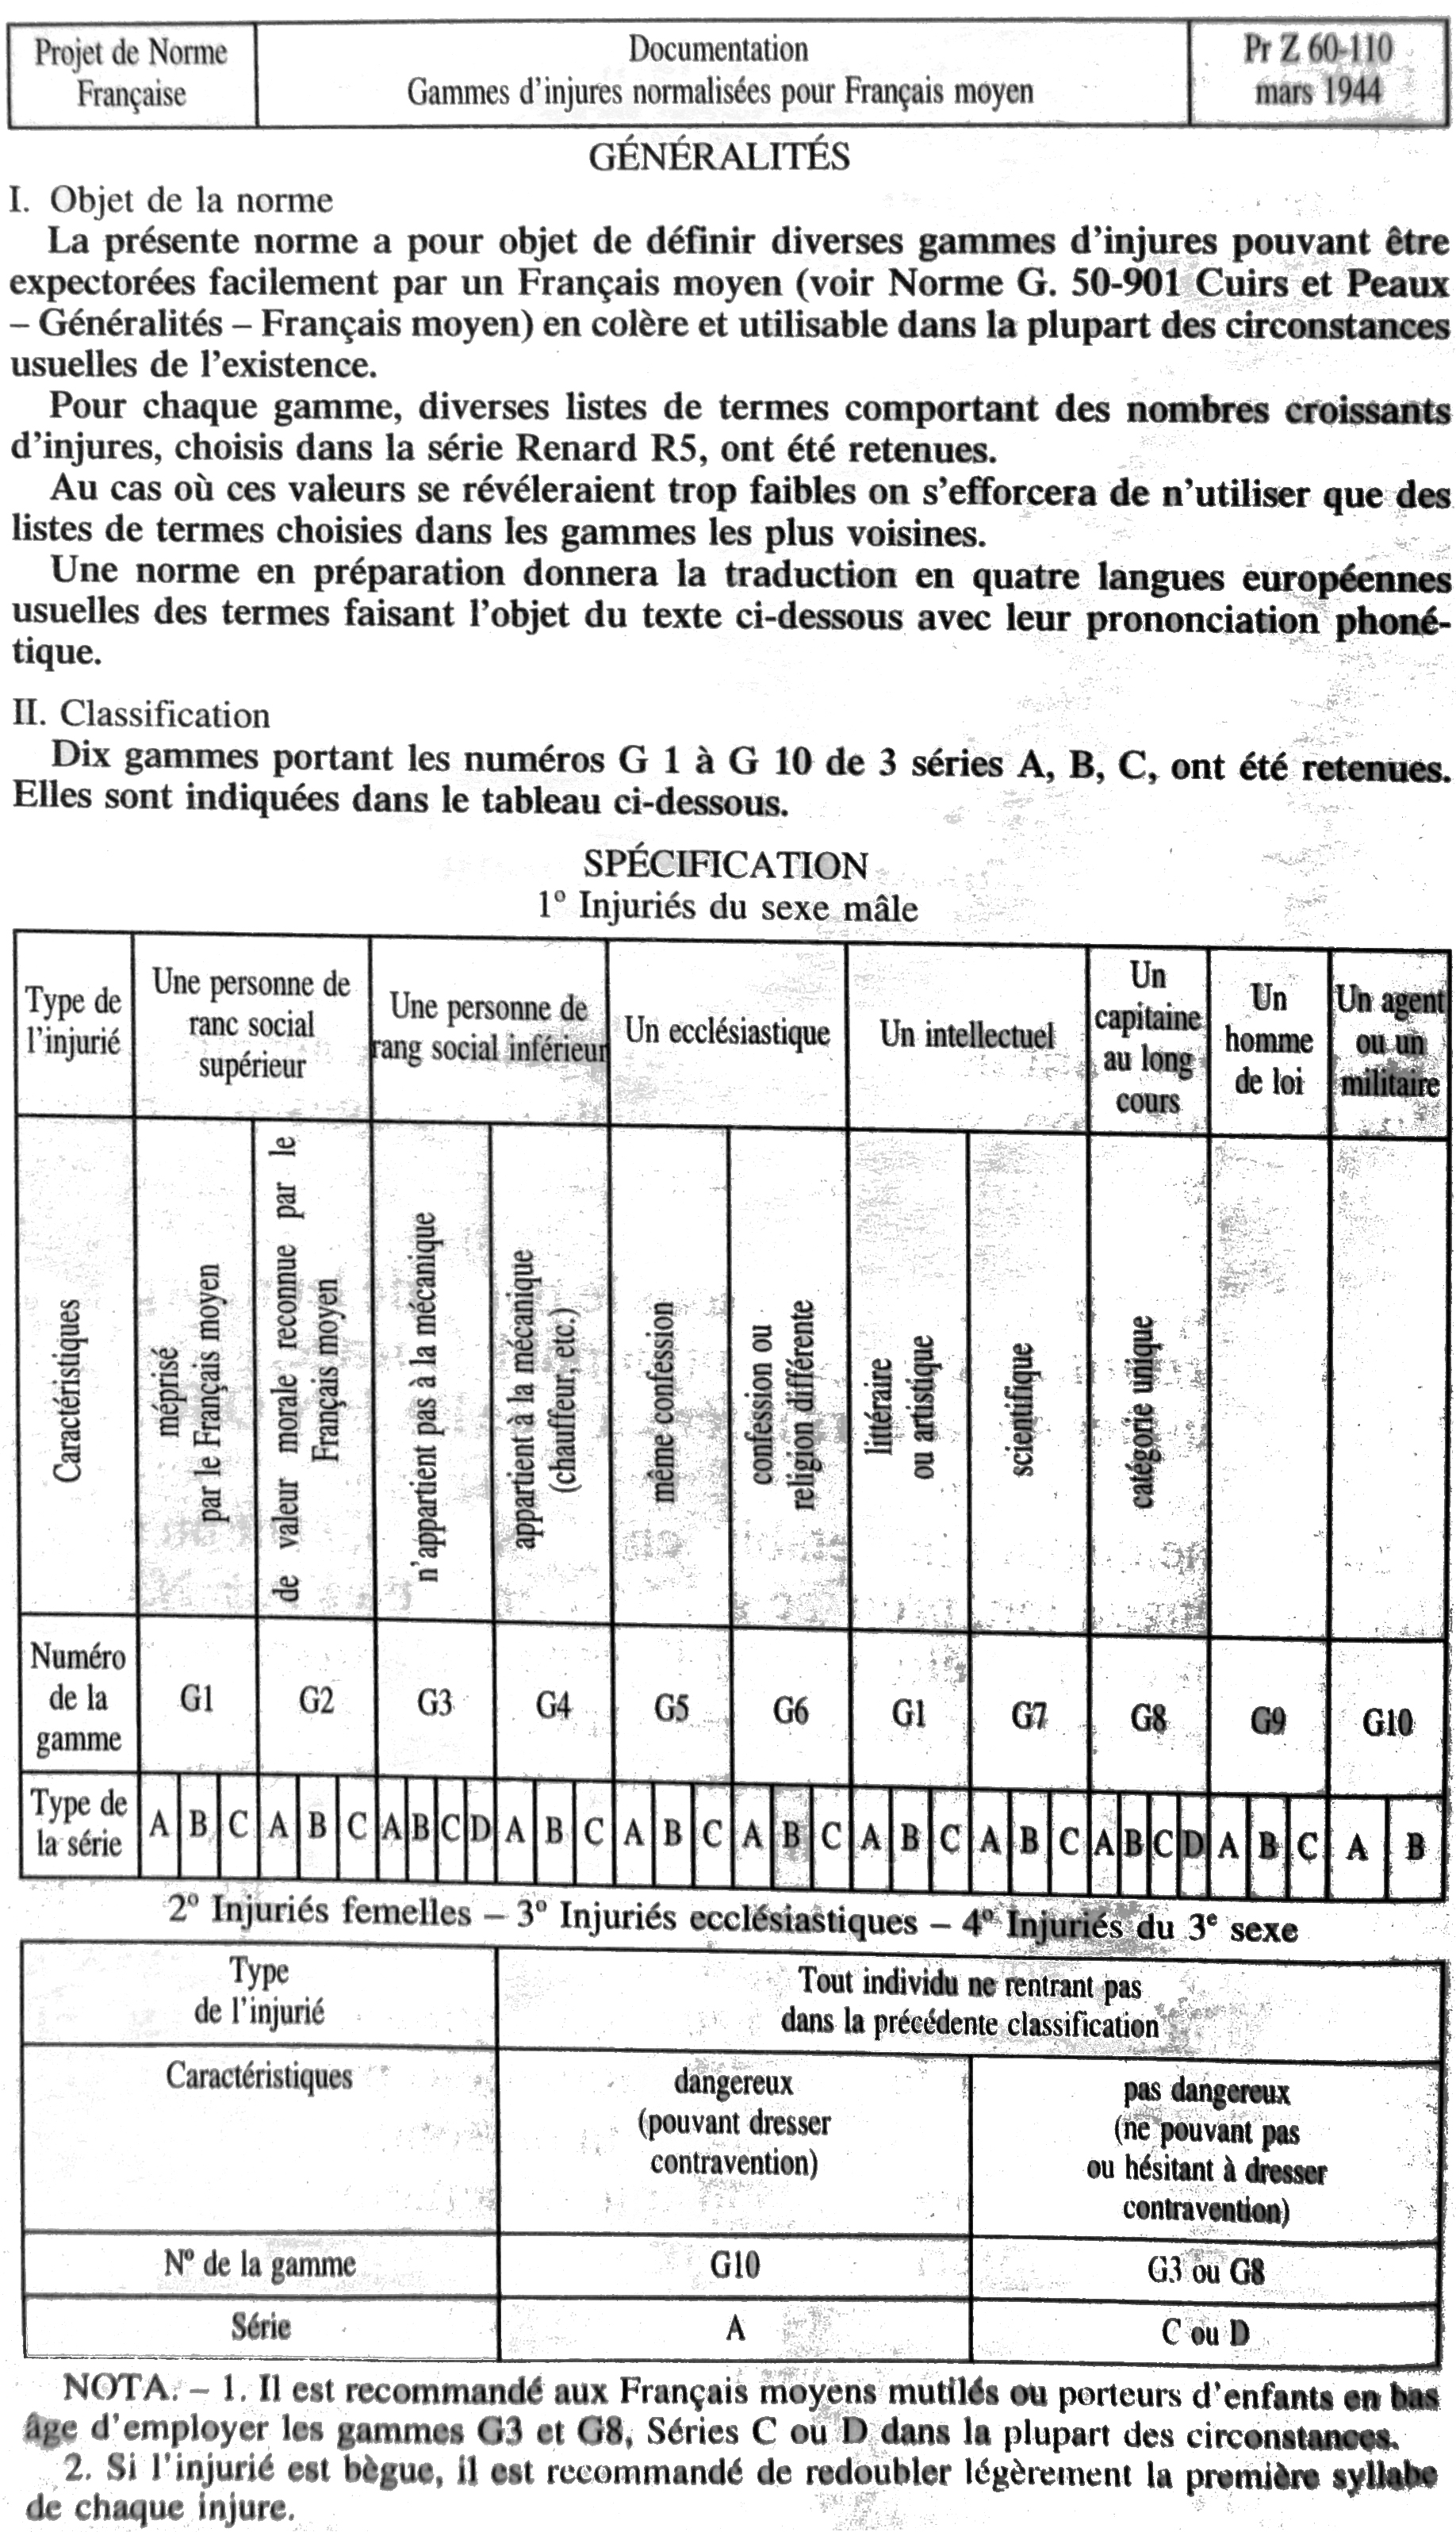
\includegraphics[height=\textheight]{\PIXPATH/ins}
\caption{Exemple de document rédigé à l'AFNOR}
\label{ins}
\end{figure}

\subsection{Le créateur}

\section{Le Jazz}
\epigraph{Il [\BV] était un amoureux du jazz, ne vivait que pour le jazz, n'entendait, ne s'exprimait qu'en jazz.}
{Henri Salvador}

\subsection{Le musicien}

\subsection{L'amateur}

\section{Le Verbe}
\epigraph{Je me demande si je ne suis pas en train de jouer avec les mots. Et si les mots étaient faits pour ça ?}
{\emph{Les Bâtisseurs d'empire}, \BV}

\subsection{Écrits}

\subsection{La pataphysique}
